\documentclass[25pt, a0paper, portrait, margin=0mm, innermargin=15mm,
     blockverticalspace=15mm, colspace=15mm, subcolspace=8mm]{tikzposter} %Default values for poster format options.

\usepackage{amsthm,amsmath,amsfonts,amssymb}
%\usepackage{pgfplots}

\theoremstyle{plain}
\newtheorem{lemma}{Lemma}

\tikzposterlatexaffectionproofoff %shows small comment on how the poster was made at bottom of poster

\renewcommand*{\familydefault}{\sfdefault}



 % Commands
 \newcommand{\bs}{\textbackslash}   % backslash
 \newcommand{\cmd}[1]{{\bf \color{red}#1}}   % highlights command

 % Title, Author, Institute
 \title{ Look Ma, No Sampling!}
 \author{Colin Fox \& Lennart Golks}
 \institute{University of Otago}
% \titlegraphic{\includegraphics[width=.15\textwidth]{unihorizcmyk-b.jpg}}

\settitle{ \vbox{ \centering
\@titlegraphic\\[\TP@titlegraphictotitledistance] 
 \color{titlefgcolor} \centering {\bfseries \Huge \@title \par} \vspace*{1em} 
{\bf\huge \@author \par} \vspace*{1em} 
{\makebox[0.1em]{\begin{minipage}[b][1em]{39.4cm} %\includegraphics[width=4cm]{/home/colin/Documents/Papers/SamplingLinearInverseProblem/Poster/qrcode.png}
	\end{minipage}}
\LARGE ISBA BayesComp Singapore 2025
\makebox[0.1em]{\begin{minipage}[b][1em]{40.2cm} \hfill %\includegraphics[width=8cm]{/home/colin/Documents/Papers/SamplingLinearInverseProblem/Poster/unihorizcmyk-b.jpg}  
\end{minipage}}
}
}}

 % -- PREDEFINED THEMES ---------------------- %
 % Choose LAYOUT:  Default, Basic, Rays, Simple, Envelope, Wave, Board, Autumn, Desert,
\usetheme{Autumn}

%\definecolorpalette{MyColorPalette}{
%    \definecolor{colorOne}{HTML}{001099}
%    \definecolor{colorTwo}{HTML}{A2C4D9}
%    \definecolor{colorThree}{HTML}{FF8533} %{F88251}
%}

%\definecolorpalette{MyColorPalette}{
%    \definecolor{colorOne}{RGB}{0,30,102}
%    \definecolor{colorTwo}{RGB}{162,196,217}
%    \definecolor{colorThree}{RGB}{255,133,41} 
%}

\definecolorpalette{MyColorPalette}{
	\definecolor{colorOne}{RGB}{86,180,233} %title color
	\definecolor{colorTwo}{RGB}{86,180,233} %background color
	%\definecolor{colorTwo}{RGB}{0,158,115} %background color
	%\definecolor{colorThree}{RGB}{230,159,0} %cite box color
	\definecolor{colorThree}{RGB}{204,121,167} %cite box color
}


\usecolorstyle[colorPalette=MyColorPalette]{Germany}
% COLORPALETTE: Default, BlueGrayOrange, GreenGrayViolet, PurpleGrayBlue, BrownBlueOrange.
% COLORSTYLE: Default, Australia, Britain, Sweden, Spain, Russia, Denmark, Germany

\newcommand{\dd}{\mathrm{d}}
\newcommand{\bbR}{\mathbb{R}}
\newcommand{\tsfrac}[2]{{\textstyle \frac{#1}{#2}}}
\newcommand{\twobyone}[2]{\begin{array}{c} #1 \\ #2 \end{array}}
\newcommand{\twobytwo}[4]{\begin{array}{cc} #1 & #2 \\ #3 & #4 \end{array}}

\newcommand{\E}{\operatorname{E}}



\begin{document}
\maketitle
%%%% title
\begin{columns}
\column{1}
\block{Tired of waiting for your MCMC to run? No problem, just skip the MCMC and evaluate expectations using function approximation and numerical integration.\\[-1.5em]}{
}
\end{columns}

\begin{columns}
\column{.6}
\begin{subcolumns}
\subcolumn{.5}
\block{Bayesian Formulation }{\vspace{-1ex}
\tikzstyle{unknown}=[circle,draw=blue!100,thick,minimum size=2.5em] %!nn appears to be how opaque as percentage
\tikzstyle{measured}=[rectangle,draw=blue!100,thick,minimum size=2.5em]
\begin{tikzpicture}%[node distance=4em]
  \node[measured] (data) {$y$};
  \node[unknown] (x)             [above of=data, node distance=4em]    {$x$};
  \node[unknown] (theta)         [above of=x, node distance=4em]          {$\theta$};
  \draw [->,very thick] (x) to (data);
  \draw [->,very thick] (theta) to (x);

  %\node (hyper) [right of=theta, node distance=6em,inner sep=0pt, align=left]  {Hyperparameters: Hyper-prior: $[\theta]$};
  \node[right of=theta, node distance=2em, inner sep=0pt, align=left, anchor=west] (hyper) {Hyperparameters: Hyper-prior: $[\theta]$};
  \node[right of=x, node distance=2em, inner sep=0pt, align=left, anchor=west] (hyper) {Latent field: Representation and prior $[x|\theta]$};
  %\node (prior) [right of=x, node distance=5em,inner sep=0pt]  {Prior model: representation and $[x|\theta]$};
  %\node (obs) [right of=data, node distance=6em,inner sep=0pt]  {Observed data: Likelihood: $[y|x]$};
  \node[right of=data, node distance=2em, inner sep=0pt, align=left, anchor=west] (obs) {Observed data: Likelihood: $[y|x]$};
\end{tikzpicture}
 The focus of inference is the posterior distribution:
%
\[ [x,\theta|y] = \frac{[y|x]\,[x|\theta]\,[\theta]}{[y]} \]
We assume the normalizing constant $[y]$ is finite.}

\subcolumn{.48}
\block{Posterior Inference}{We wish to compute expectations:
\coloredbox{\[ \E_{x,\theta|y}[f(x)] = \int f(x) [x,\theta|y]\,\dd x\,\dd\theta \]}}

\block{Notation}{
We learned this notation from Alan Gelfand: read $[a]$ as ``the distribution over $a$'', and $[a|b]$ as ``the distribution over $a$ given $b$''. We will abuse this notation to also denote the density function.
}

\end{subcolumns}

\block{Factorize Posterior (MTC)}{
factorisation of the posterior density
\[ [x,\theta|y] = [x|\theta,y]\,[\theta|y] \]
i.e. into the full conditional for $x$ and the marginal posterior over $\theta$.

% \begin{lemma}
%\label{lem:mtc}
\textbf{Lemma} Sampling $\theta'\sim [\theta|y]$ then $x'\sim [x|\theta',y]$
generates a sample from the posterior distribution, i.e.,
\[ \left(x' ,\theta'\right) \sim [x,\theta|y]. \]
% \end{lemma}

\coloredbox{
C.~Fox and R.~A. Norton.
\newblock Fast sampling in a linear-Gaussian inverse problem.
\newblock {\em SIAM/ASA Journal on Uncertainty Quantification},
  4(1):1191--1218, 2016.
}
}

\block{Marginal Posterior over Hyperparameters }{
The marginal posterior distribution over hyperparameters is defined by the integral $[\theta|y]=\int_X [x,\theta|y]\,\dd x$, as mentioned above, but this calculation is to be avoided because the integral is over the high-dimensional latent field $x$. %, with cost exacerbated when we are interested in the limit of infinite dimensional $x$.
A cheap algebraic calculation is available when the full conditional for $x$
\[ [x | \theta, y] = \frac{[ y | x]\,[ x | \theta ]}{[y|\theta]} \]
has known form, implying that the normalising constant $[y|\theta]$ has known $\theta$ dependence, and hence one can evaluate the marginal posterior over $\theta$
\[ [\theta | y] \propto [ y | \theta][\theta]. \]
\coloredbox{
R.~A. Norton, J.~A. Christen, and C.~Fox.
\newblock Sampling hyperparameters in hierarchical models: improving on {Gibbs}
  for high-dimensional latent fields and large datasets.
\newblock {\em Communications in Statistics - Simulation and Computation},
  47(9):2639--2655, 2018.
}
}
\note[targetoffsetx=0.17\textwidth,targetoffsety=9cm,innersep=.4cm,angle=-45,connection,radius=5cm]{These terms simplify when $A^{-1}b = \mathcal{A}^{-1}\beta$}

% \note[targetoffsetx=1cm, targetoffsety=-1.5cm,rotate=2,angle=270,radius=8cm,width=.5\textwidth,innersep=.4cm]{
% {\large A jaunty note.}
% }


\column{.4}
\block{Monte Carlo Integration}{{~}\\[-3em]
\begin{align*}
 \E_{x,\theta|y}[f(x)] %&= \int f(x) \pi(x,\theta|y)\,\dd x\dd\theta\\
                     &\approx \frac{1}{N}\sum_{i=1}^N f(x_i)
\end{align*}
where %$(x_i,\theta_i)\sim \pi(x,\theta|y)$, or more generally
$\left\{(x_i,\theta_i)\right\}$ is ergodic for $[x,\theta|y]$.
\coloredbox{
\begin{quotation}
 ``Monte Carlo is an extremely bad method; it should be used only when all alternative methods are worse.'' (Alan Sokal)
\end{quotation}
}
}


% \end{columns}
%
% \begin{columns}
% \column{0.6}
%
%
%
%
% \column{0.4}
\block{Markov chain Monte Carlo}{
A representative MCMC scheme is the block Gibbs sampler %that updates  $(x,\theta)$ to $(x',\theta')$ by alternating drawing from full conditionals
\begin{itemize}
 \item Draw $\theta'\sim [\theta|x]$
 \item Draw $x' \sim [x|\theta',y]$
\end{itemize}
simulating a transition kernel that targets the posterior $[x,\theta|y]$.\\
\centerline{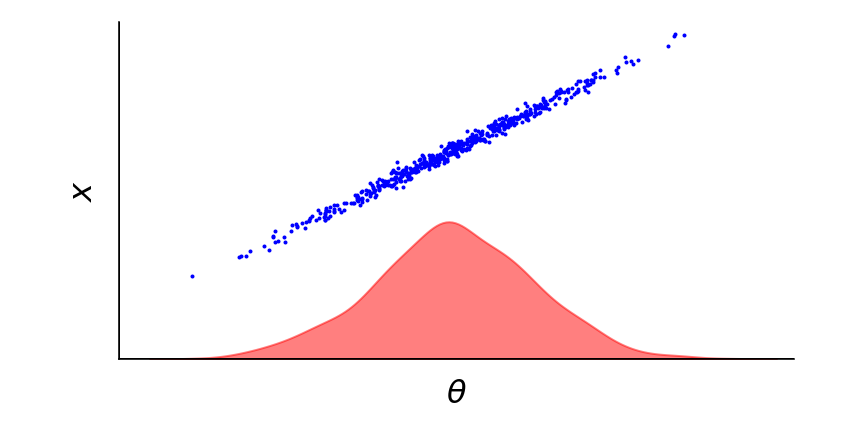
\includegraphics[]{scatterplotmarginal.png}}
Narrow scatter plot shows why this is slow
\coloredbox{Better is to move in the marginal posterior over hyperparameters $[\theta|y]$\\
            H.~Rue and L.~Held.
\newblock {\em Gaussian {M}arkov random fields : {T}heory and applications}.
\newblock Chapman Hall, New York, 2005.}
}

\block{Some kind of pictorial break}{But not a box with text like this}

\block{Tensor Train Representation of PDF}{
\centering
A surface rendering of a density in TT format \\ TT formula
\coloredbox{S.~Dolgov, K.~Anaya-Izquierdo, C.~Fox, and R.~Scheichl.
\newblock Approximation and sampling of multivariate probability distributions
  in the tensor train decomposition.
\newblock {\em Statistics and Computing}, 30(3):603--625, 2020. }
}
\end{columns}

\begin{columns}
\column{.45}
\block{Inverse Problem of Recovering Ozone Profile }{I'm thinking picture of satellite, DAG, RTE
}

\note[targetoffsetx=-8cm, targetoffsety=-12cm,radius=8cm,width=.48\textwidth,innersep=1cm]{
R. A. Norton and C. Fox, Efficiency and computability of MCMC with Langevin, Hamiltonian, and other matrix-splitting proposals, arxiv:1501.03150.
}


\column{.55}
\block{Posterior Expectation by TT  and Affine Representations}{Picture of posterior inference, or timings, or some output summaries -- perhaps a box below with some snappy summary or conclusions
}
\end{columns}

\end{document}

\endinput
%%
